\documentclass[11pt]{article}

\usepackage[a4paper,margin=1in]{geometry}
\usepackage{graphicx}
\usepackage{booktabs}
\usepackage{array}
\usepackage{tabularx}
\usepackage{amsmath}
\usepackage{amssymb}
\usepackage{siunitx}
\usepackage{multirow}
\usepackage{caption}
\usepackage{subcaption}
\usepackage{float}
\usepackage{hyperref}
\usepackage[authoryear]{natbib}

\hypersetup{
  colorlinks=true,
  linkcolor=blue,
  citecolor=blue,
  urlcolor=blue
}

\title{Inflammation-Linked Aging Signals in Frozen Single-Cell Foundation Models: Donor-Aware Detection and Robustness Testing}
\author{Ihor Kendiukhov$^{1}$\\$^{1}$Department of Computer Science, University of T\"ubingen, T\"ubingen, Germany\\\texttt{kendiukhov@gmail.com}}
\date{}

\begin{document}
\maketitle

\begin{abstract}
Single-cell foundation models offer a possible route to studying aging biology in latent space, but apparent age effects can be distorted by donor identity and cell-composition differences. We developed a donor-aware interpretability workflow to test whether frozen scGPT and Geneformer representations contain biologically coherent aging signals in age-labeled human single-cell datasets. The workflow combined donor-held-out age decoding, sparse autoencoder feature discovery, cross-model pathway matching, targeted latent-space interventions, donor-bootstrap confidence intervals, and progressively stricter confound controls.

Across five datasets, frozen representations contained detectable age information, with best donor-aware balanced accuracy of 0.384. Sparse autoencoders identified 132 donor-aware robust features, and cross-model pathway matching produced 193 paired features, with the strongest convergence in inflammation and NF-kappaB-related programs. The clearest intervention signal was observed in a global Geneformer inflammatory branch, where old-versus-random and old-versus-young contrasts remained positive after split expansion and donor-threshold tightening up to 400 donors. In a monocyte-restricted analysis, both scGPT and Geneformer also showed positive old-versus-random responses in one cohort.

The strongest global signal weakened under stricter controls. Fully composition-matched forward-pass reruns yielded 0 of 4 full strict replications. These results indicate that frozen single-cell foundation models do capture biologically plausible aging-related structure, especially around inflammatory programs, but also that donor-aware and composition-aware stress tests are necessary before interpreting such signals as robust mechanisms.
\end{abstract}

\noindent\textbf{Keywords:} aging; inflammaging; single-cell transcriptomics; foundation models; interpretability; immune aging

\section{Introduction}
Aging is now understood as a systems-level process rather than a single molecular clock, with recurring hallmarks that include chronic inflammation, senescence-associated secretory signaling, stem-cell dysfunction, impaired proteostasis, and altered intercellular communication \citep{lopez2013hallmarks,lopez2023hallmarks,kennedy2014geroscience,campisi2019therapeutics}. In immune and stromal compartments, age-related inflammation is especially prominent. The inflammaging literature links late-life dysfunction to persistent innate immune activation, NF-kappaB signaling, senescence-associated secretory phenotypes, and age-related rewiring of adaptive immunity \citep{franceschi2000inflammaging,fabbri2014chronic,furman2019chronic,ferrucci2018inflammageing,nikolich2018twilight,goronzy2019tcell,salminen2008nfkb,chien2011sasp,hernandez2018senescence,basisty2020secretome,zhang2013hypothalamic}.

At the measurement level, aging can often be detected from molecular profiles, including DNA methylation clocks, blood transcriptomic signatures, and large atlas-scale single-cell references \citep{horvath2013age,lu2019grimage,peters2015bloodage,tabulamuris2020,schaum2020hallmarks,tabula2022,yazar2022}. What remains unclear is whether compact latent representations learned by large models encode merely enough information for age prediction, or whether they contain interpretable biological programs that track conserved aging mechanisms.

Single-cell foundation models provide a concrete setting in which to test that distinction. Transformer architectures have become the dominant substrate for large representation learners \citep{vaswani2017attention}, and recent biological variants such as Geneformer and scGPT show that frozen transformer backbones can organize rich cellular structure in transcriptomic data \citep{theodoris2023geneformer,cui2024scgpt}. In parallel, mechanistic-interpretability work has developed increasingly structured ways to study latent circuits and sparse features in large models \citep{olah2020circuits,bau2017network,bricken2023monosemanticity,templeton2024scaling}. Together, these developments motivate a harder question for biogerontology: do frozen single-cell foundation models encode aging biology in a form that survives mechanistic scrutiny?

This distinction matters because age can be decodable without supporting a defensible biological mechanism. Donor identity, cell-type imbalance, and cohort-specific composition shifts can all create apparent aging signals that disappear under stronger controls. We therefore focused on a harder target: not just whether age can be decoded from frozen embeddings, but whether candidate aging programs remain directional, biologically coherent, and donor-aware under increasingly strict stress tests.

\section{Methods}
\subsection{Data}
Core analyses centered on age-labeled human immune single-cell data already available in-project, with primary focus on two internal AIDA immune-aging cohorts. External and reference datasets included Tabula Sapiens-derived assets \citep{tabula2022}, the Yazar immune single-cell eQTL cohort \citep{yazar2022}, and Allen immune aging-derived subsets. We treated atlas-scale external datasets primarily as stress-test context rather than as interchangeable pooled training data, because cross-cohort integration in single-cell studies is sensitive to normalization choices, batch effects, missingness, donor structure, and pseudoreplication \citep{luecken2019bestpractices,wolf2018scanpy,hafemeister2019sctransform,stuart2019integration,haghverdi2018mnn,korsunsky2019harmony,tran2020batch,hicks2018missing,zimmerman2021pseudoreplication,squair2021false}.

The strongest-branch analyses were performed on the larger of the two AIDA cohorts, which had the greatest donor support in the deep-dive analysis (\(n\approx 424\) in the baseline expanded-split run and \(n\approx 333\)--340 in the composition-matched reruns).

\subsection{Models}
We used frozen representations from:
\begin{itemize}
  \item \textbf{scGPT} (contextual layer \texttt{scgpt\_layer\_09}) \citep{cui2024scgpt}
  \item \textbf{Geneformer} (contextual representation) \citep{theodoris2023geneformer}
\end{itemize}

Neither model was fine-tuned for age prediction in the core pipeline.

\subsection{Interpretability workflow}
The analysis proceeded in four blocks. First, we asked whether age-related signal was present at all, using donor-held-out linear probes and simple manifold diagnostics. Second, we searched for interpretable latent structure using sparse autoencoders and cross-model pathway matching, motivated by sparse dictionary learning frameworks \citep{bricken2023monosemanticity,templeton2024scaling}. Third, we tested candidate pathways with targeted interventions, donor-bootstrap confidence intervals, and conservative promotion criteria. Finally, we stress-tested the strongest surviving branch with donor-threshold sweeps, donor-composition reweighting, fully composition-matched reruns, and multi-seed matched reruns.

Bootstrap confidence intervals used nonparametric donor resampling \citep{efron1979bootstrap}.

\subsection{Statistical safeguards}
Single-cell datasets are unusually vulnerable to optimistic results when cells are treated as independent evidence, when donor effects leak across splits, or when batch correction silently redefines the tested biological contrast \citep{crowell2020muscat,zimmerman2021pseudoreplication,squair2021false}. For that reason, the pipeline was built around donor-aware data partitioning, donor-bootstrap uncertainty estimates, and contrast checks that remained interpretable after composition reweighting or composition-matched reruns. The goal was not to maximize nominal detection rate, but to suppress exactly the kinds of confounded positives that are common in atlas-scale analyses \citep{luecken2019bestpractices,tran2020batch,hicks2018missing}.

\subsection{Strict gate policy}
Claims were promoted only when multiple directional checks agreed: expected-age contrasts had to point in the correct direction, marginal effects had to remain supportive, and old-probability shifts had to be consistent. This policy was intentionally stricter than contrast-only screening because the project goal was mechanism-grade evidence rather than loose signal detection.

\section{Results}
\subsection{Global trajectory across the analysis pipeline}
Table~\ref{tab:stage-overview} summarizes the main outcomes across the pipeline.

\begin{table}[H]
\centering
\small
\caption{Analysis outcomes across the full pipeline.}
\label{tab:stage-overview}
\begin{tabularx}{\textwidth}{p{1.8cm}p{3.0cm}X}
\toprule
\textbf{Block} & \textbf{Objective} & \textbf{Key outcome} \\
\midrule
1 & Frozen age probe & Best balanced accuracy range: 0.299--0.384 across 5 datasets \\
2 & Manifold geometry & Geometry gate passes: 0/5 datasets \\
3 & SAE features & 132 robust donor-aware sparse features retained \\
4 & Cross-model convergence & 193 pathway-matched cross-model feature pairs \\
6 (strict) & Model-specific claim promotion & 0/4 strict claim passes \\
8 (strict audit) & Contrast + marginal strict gate & 1/19 runs with at least one full strict row \\
9 & Deep-dive robustness & Surviving row stable up to min-donors=400; fails at 500 \\
10 & Composition controls & Reweighting preserved strict pass; full compmatched forward rerun removed full strict pass \\
11 & Compmatched seed panel & 0/4 full strict replications under composition-matched seeds \\
\bottomrule
\end{tabularx}
\end{table}

\subsection{Age can be decoded, but global age geometry is not robust}
Frozen probes reached moderate performance (best \(\mathrm{BA}=0.3838\) in AIDA phase 1 v2), indicating that age-associated signal is present in the frozen representations. However, the manifold-alignment criteria did not pass robustness gates in any dataset (0/5), even after donor-aware within-cell-type checks. Figure~\ref{fig:stage12} shows this separation clearly: age is detectable, but it does not organize the global latent geometry in a stable way.

\begin{figure}[H]
\centering
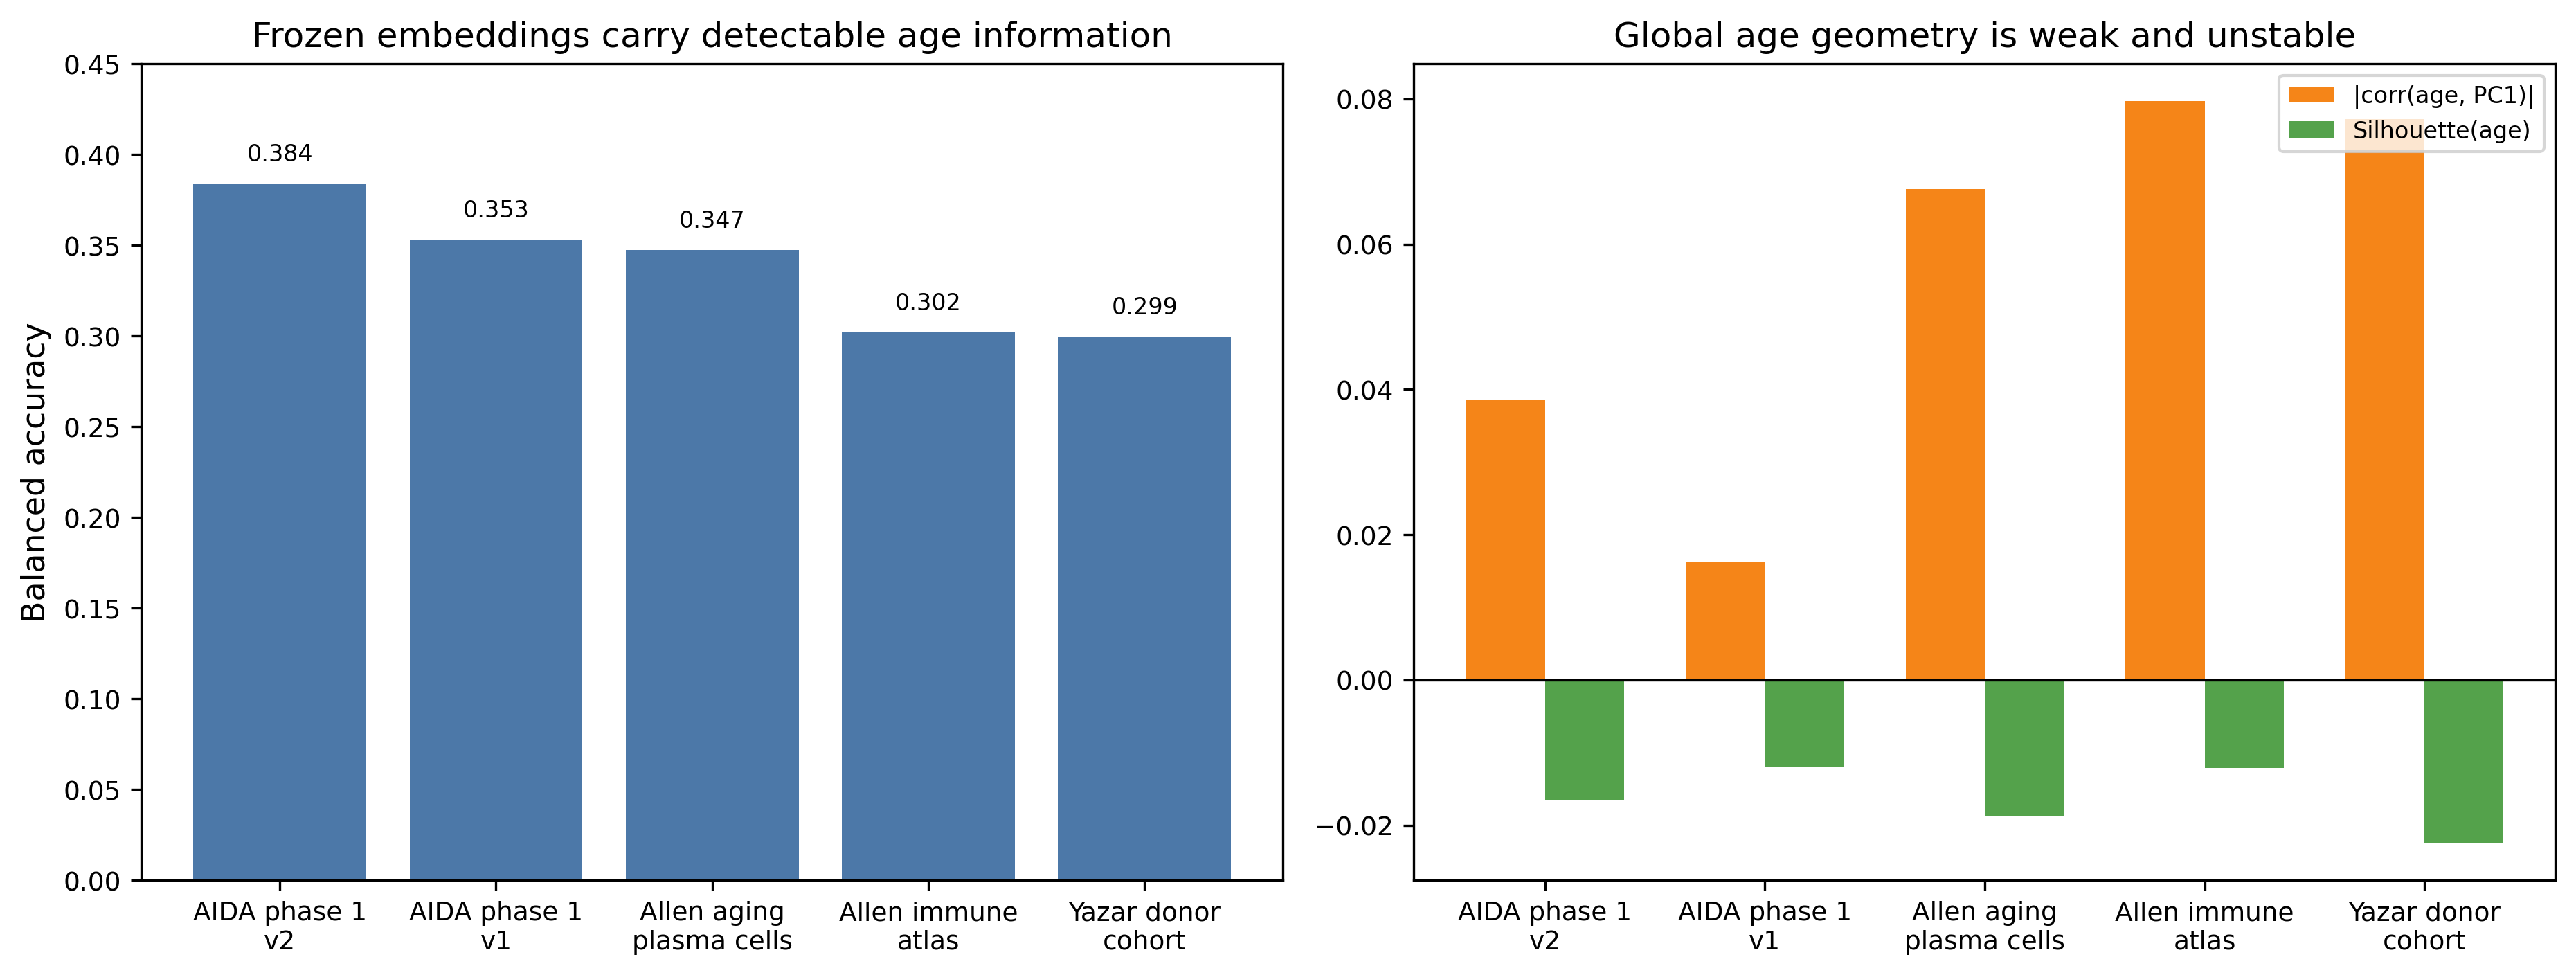
\includegraphics[width=0.98\textwidth]{figures/fig1_stage1_stage2_overview.png}
\caption{Detection versus geometry. Left: donor-aware age-decoding performance by dataset. Right: age-alignment geometry statistics remain weak and inconsistent, with no dataset passing the geometry gate.}
\label{fig:stage12}
\end{figure}

\subsection{Sparse features and cross-model overlap point to inflammatory programs}
Sparse autoencoder analysis identified many donor-aware robust features (91 in scGPT core runs and 41 in Geneformer core runs). Figure~\ref{fig:stage3} summarizes these counts.

\begin{figure}[H]
\centering
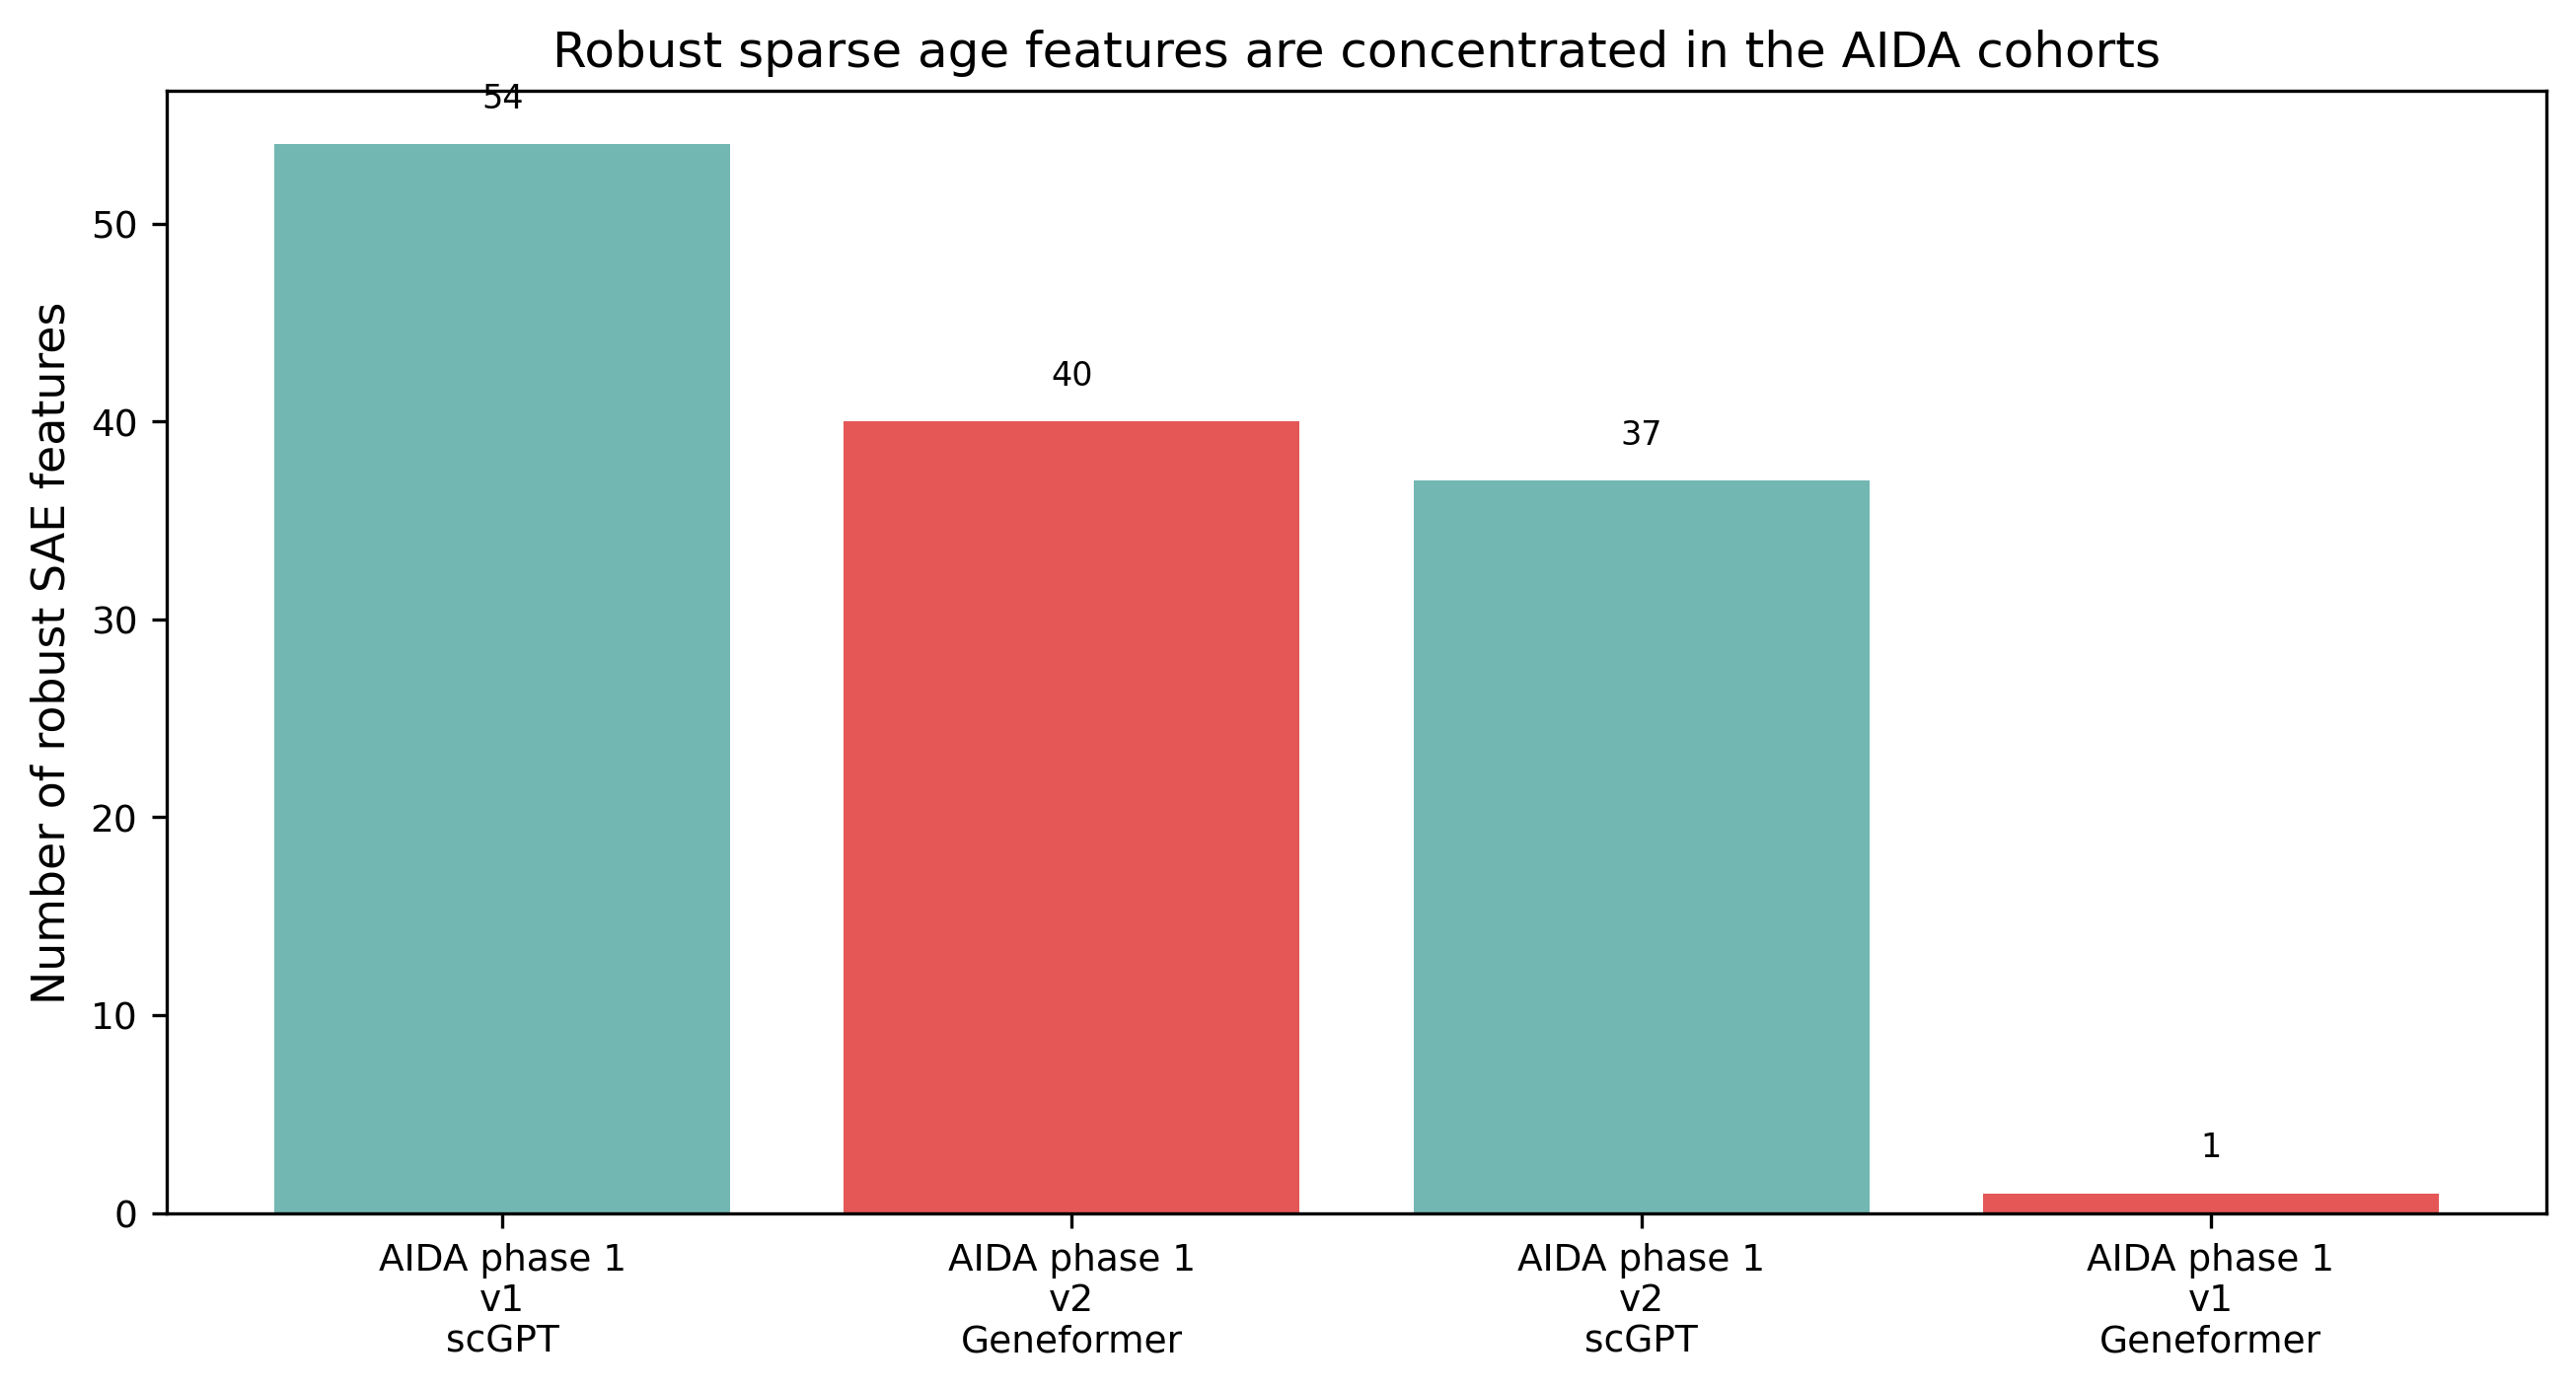
\includegraphics[width=0.75\textwidth]{figures/fig2_stage3_robust_features.png}
\caption{Donor-aware robust sparse features retained after filtering. Most of the signal comes from the two AIDA cohorts.}
\label{fig:stage3}
\end{figure}

Cross-model pathway matching produced 193 pairs in aggregate. This overlap was dominated by inflammation / NF-kappaB in AIDA phase 1 v2 (175 pairs; best convergence score 0.0957), suggesting that both models capture a shared inflammatory latent program rather than completely unrelated features (Figure~\ref{fig:stage4}).

\begin{figure}[H]
\centering
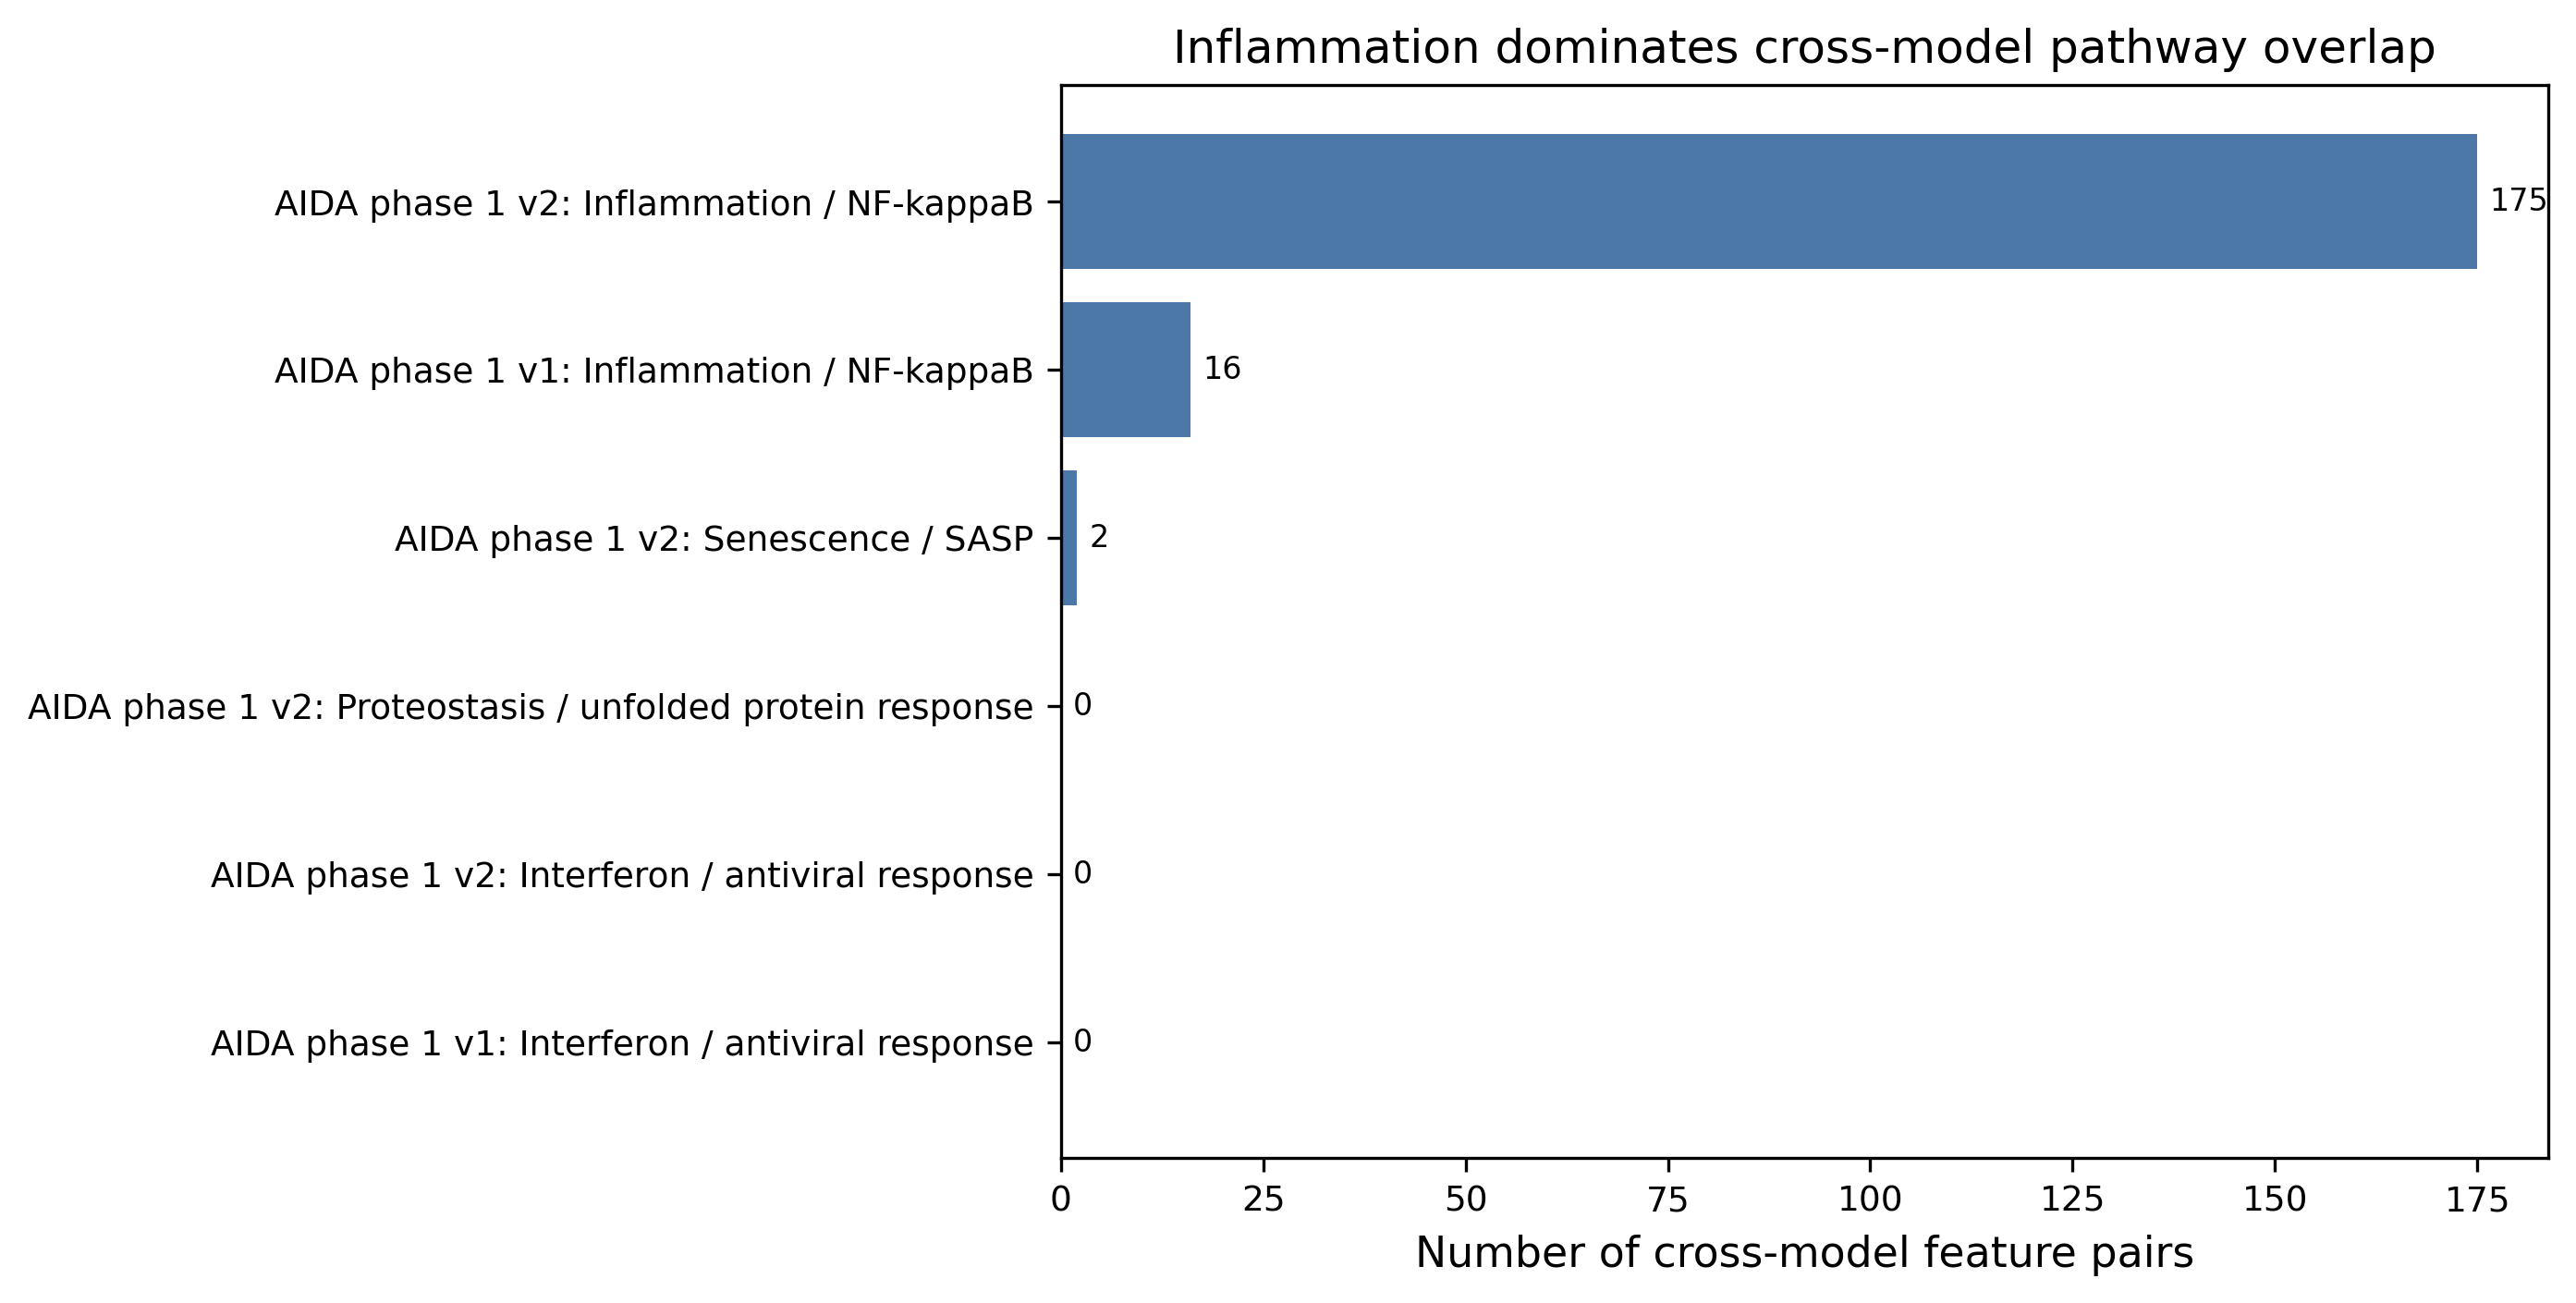
\includegraphics[width=0.80\textwidth]{figures/fig3_stage4_pathway_convergence.png}
\caption{Cross-model pathway convergence. Inflammation / NF-kappaB dominates the shared signal between scGPT and Geneformer.}
\label{fig:stage4}
\end{figure}

\subsection{The clearest cell-type-specific signal appears in AIDA v1 monocytes}
A clear positive result appeared in AIDA phase 1 v1 CD14 monocytes for inflammation / NF-kappaB at intervention scale 2.0:
\begin{itemize}
  \item Geneformer old-minus-random expected-age contrast: 0.0357 [0.0314, 0.0398], positive.
  \item scGPT old-minus-random expected-age contrast: 0.0419 [0.0368, 0.0474], positive.
\end{itemize}
In contrast, AIDA phase 1 v2 monocytes were weak or discordant (Geneformer uncertain; scGPT negative), emphasizing that the signal is real but cohort-dependent (Figure~\ref{fig:stage8}).

\begin{figure}[H]
\centering
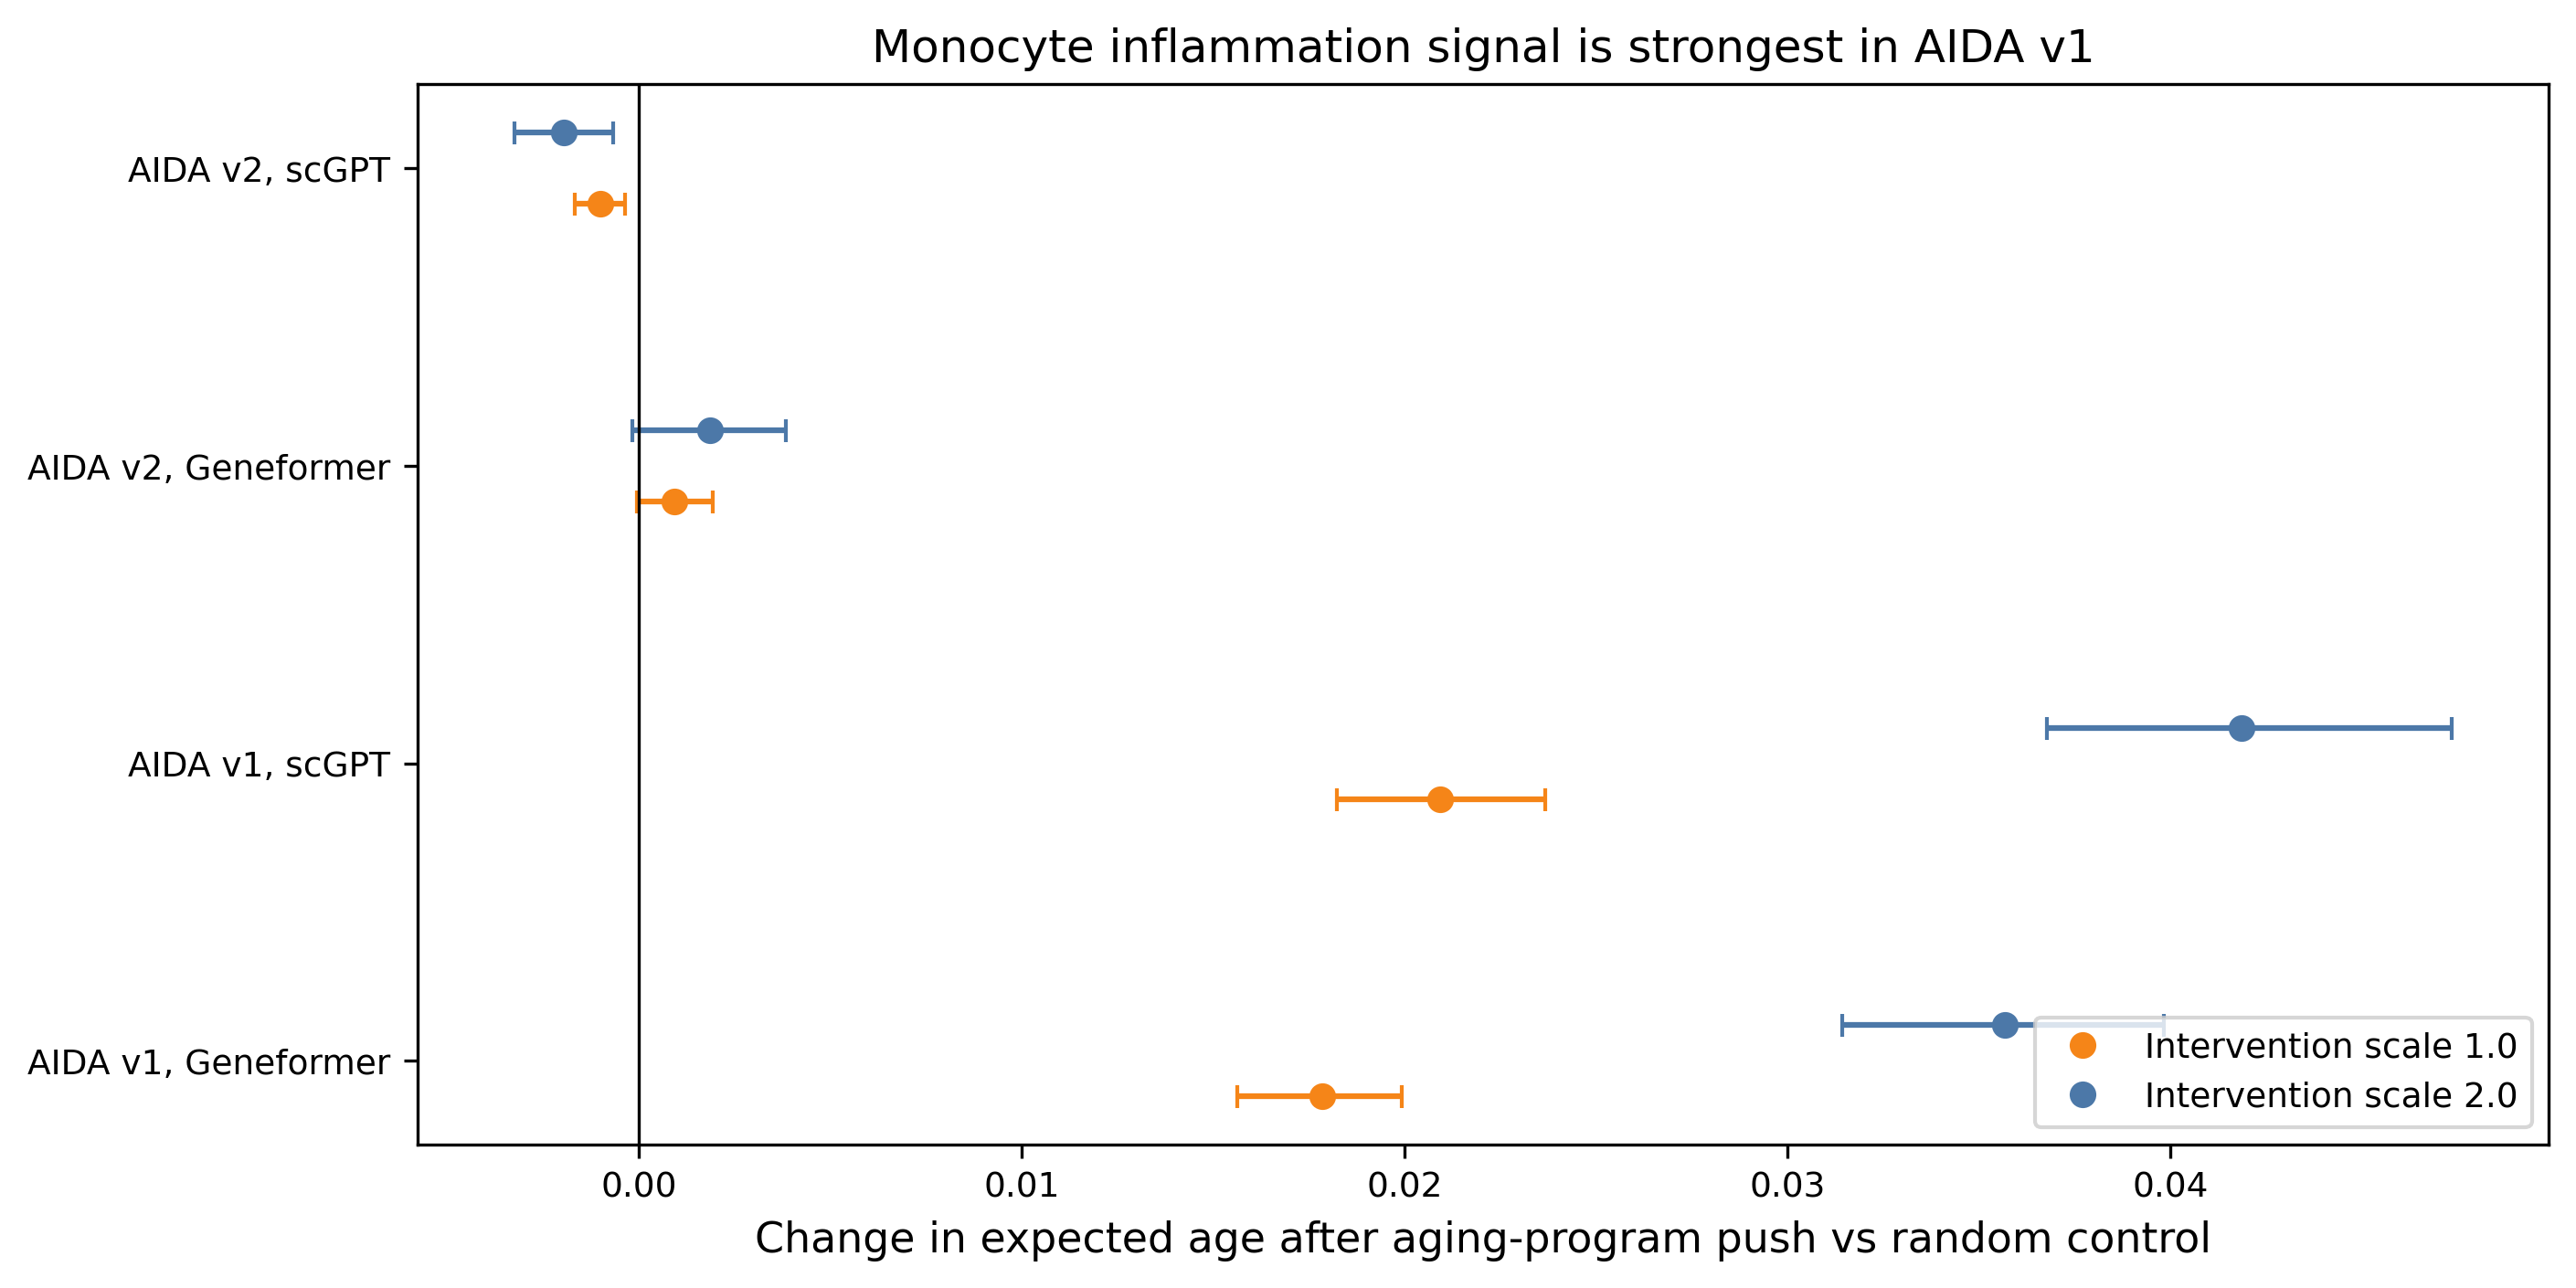
\includegraphics[width=0.90\textwidth]{figures/fig4_stage8_monocyte_scale_contrast.png}
\caption{Monocyte-restricted inflammation intervention results. Positive old-versus-random effects are strongest in AIDA phase 1 v1, especially at intervention scale 2.0.}
\label{fig:stage8}
\end{figure}

\subsection{A single global Geneformer branch survives the deep-dive stress test}
Under strict gating, one global branch survived: the AIDA phase 1 v2 Geneformer inflammation / NF-kappaB branch evaluated at global scope and intervention scale 2.0. After expanding split seeds (60 splits per model), this branch remained full-strict positive up to a minimum donor threshold of 400, failing only at 500 because donor coverage became too sparse (Figure~\ref{fig:stage9sweep}).

The key Geneformer expected-age contrasts in this deep-dive run were:
\begin{itemize}
  \item old-minus-random: 0.1494 [0.1423, 0.1564], positive
  \item young-minus-random: -0.1324 [-0.1379, -0.1267], negative
  \item old-minus-young: 0.2817 [0.2698, 0.2940], positive
\end{itemize}

This was the strongest positive mechanistic candidate in the full project trajectory.

\begin{figure}[H]
\centering
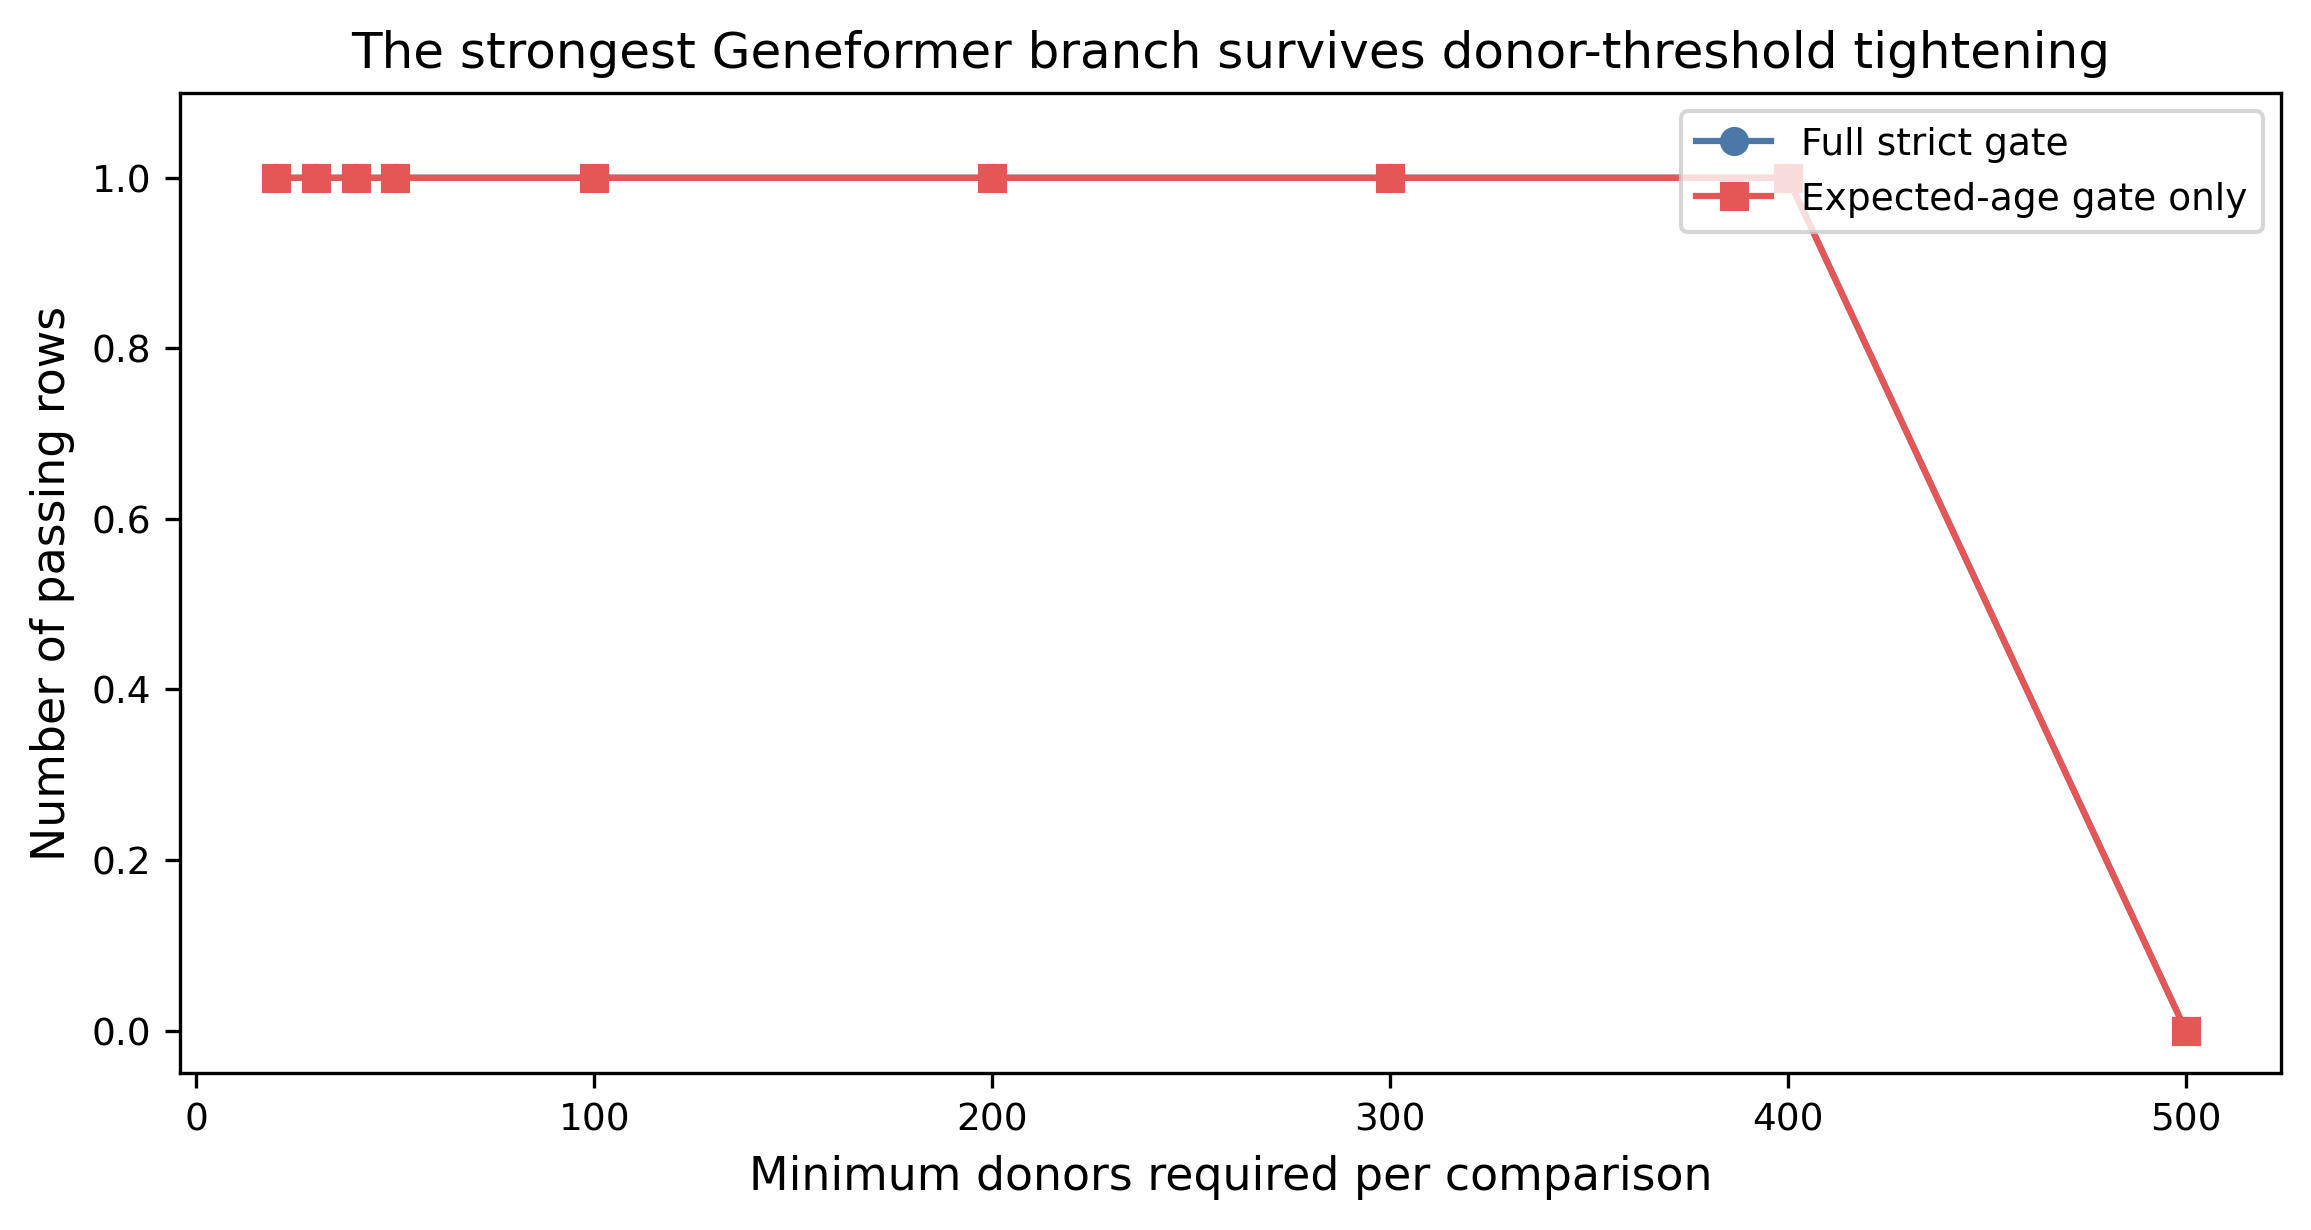
\includegraphics[width=0.72\textwidth]{figures/fig5_stage9_donor_threshold_sweep.png}
\caption{Donor-threshold stress test for the strongest surviving global branch. The full strict gate remains satisfied until the minimum donor threshold reaches 500.}
\label{fig:stage9sweep}
\end{figure}

\subsection{Composition matching weakens the strongest global signal}
\textbf{Positive control result (reweighting):} donor-composition reweighting preserved strict pass status across ridge penalties of 0.1, 1, 10, and 100, with near-zero effect shifts.

\textbf{Stronger control result (full composition-matched forward rerun):} the full strict pass disappeared (\(n_{\mathrm{full\ strict}}=0\)) despite one expected-age contrast-strict row. Figure~\ref{fig:stage10_11} shows both points: simple reweighting barely changes the estimated effect sizes, but fully matched reruns do not preserve the baseline claim. Figure~\ref{fig:bootcompare} compares the donor-bootstrap intervention intervals before and after full composition matching.

\begin{figure}[H]
\centering
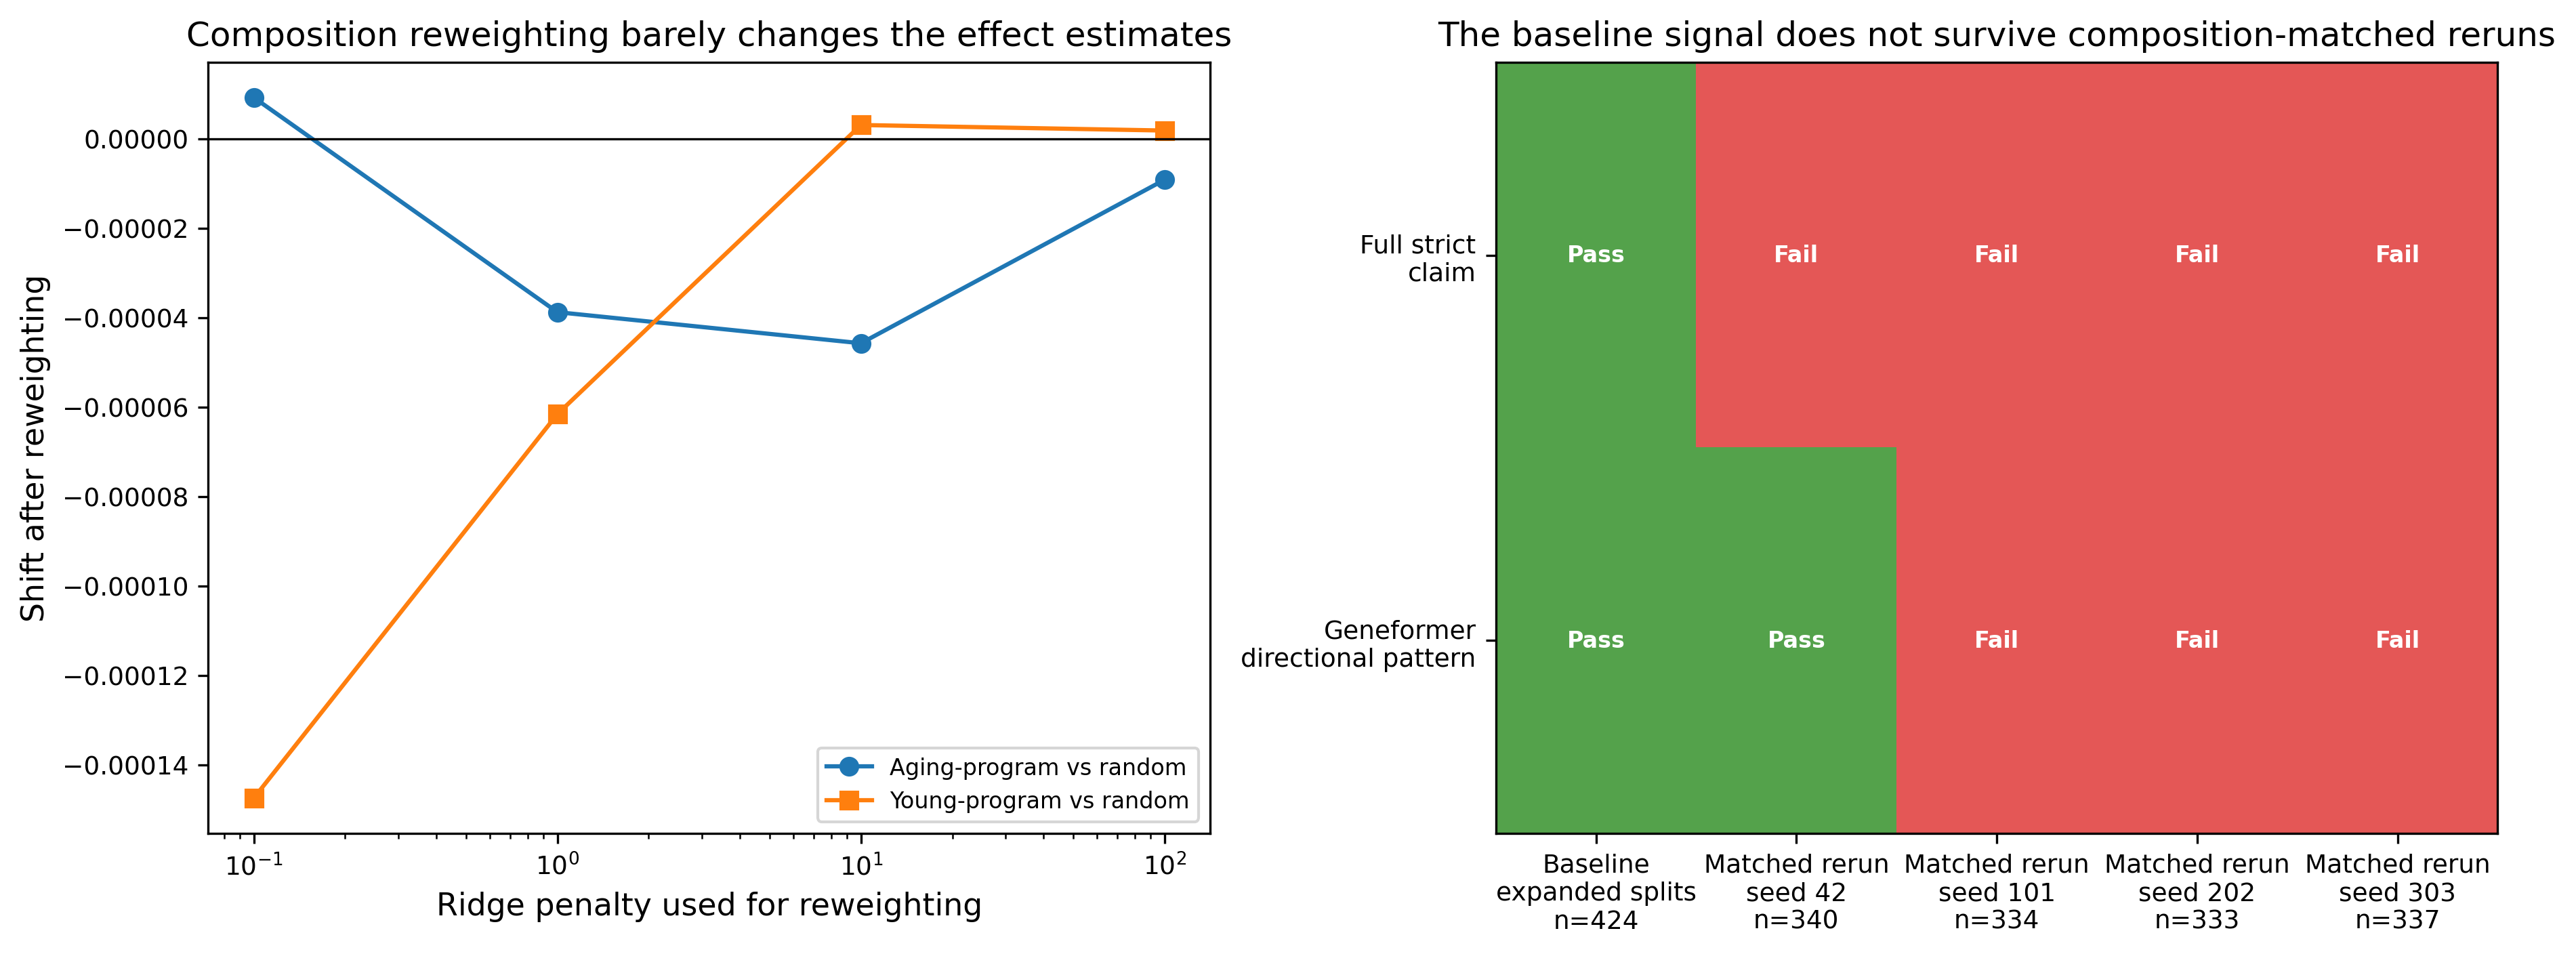
\includegraphics[width=0.98\textwidth]{figures/fig6_composition_controls_and_seedpanel.png}
\caption{Composition controls. Left: donor-composition reweighting produces only negligible changes in the effect estimates. Right: the baseline strict claim does not replicate under composition-matched reruns, although one matched rerun retains the weaker Geneformer directional pattern.}
\label{fig:stage10_11}
\end{figure}

\begin{figure}[H]
\centering
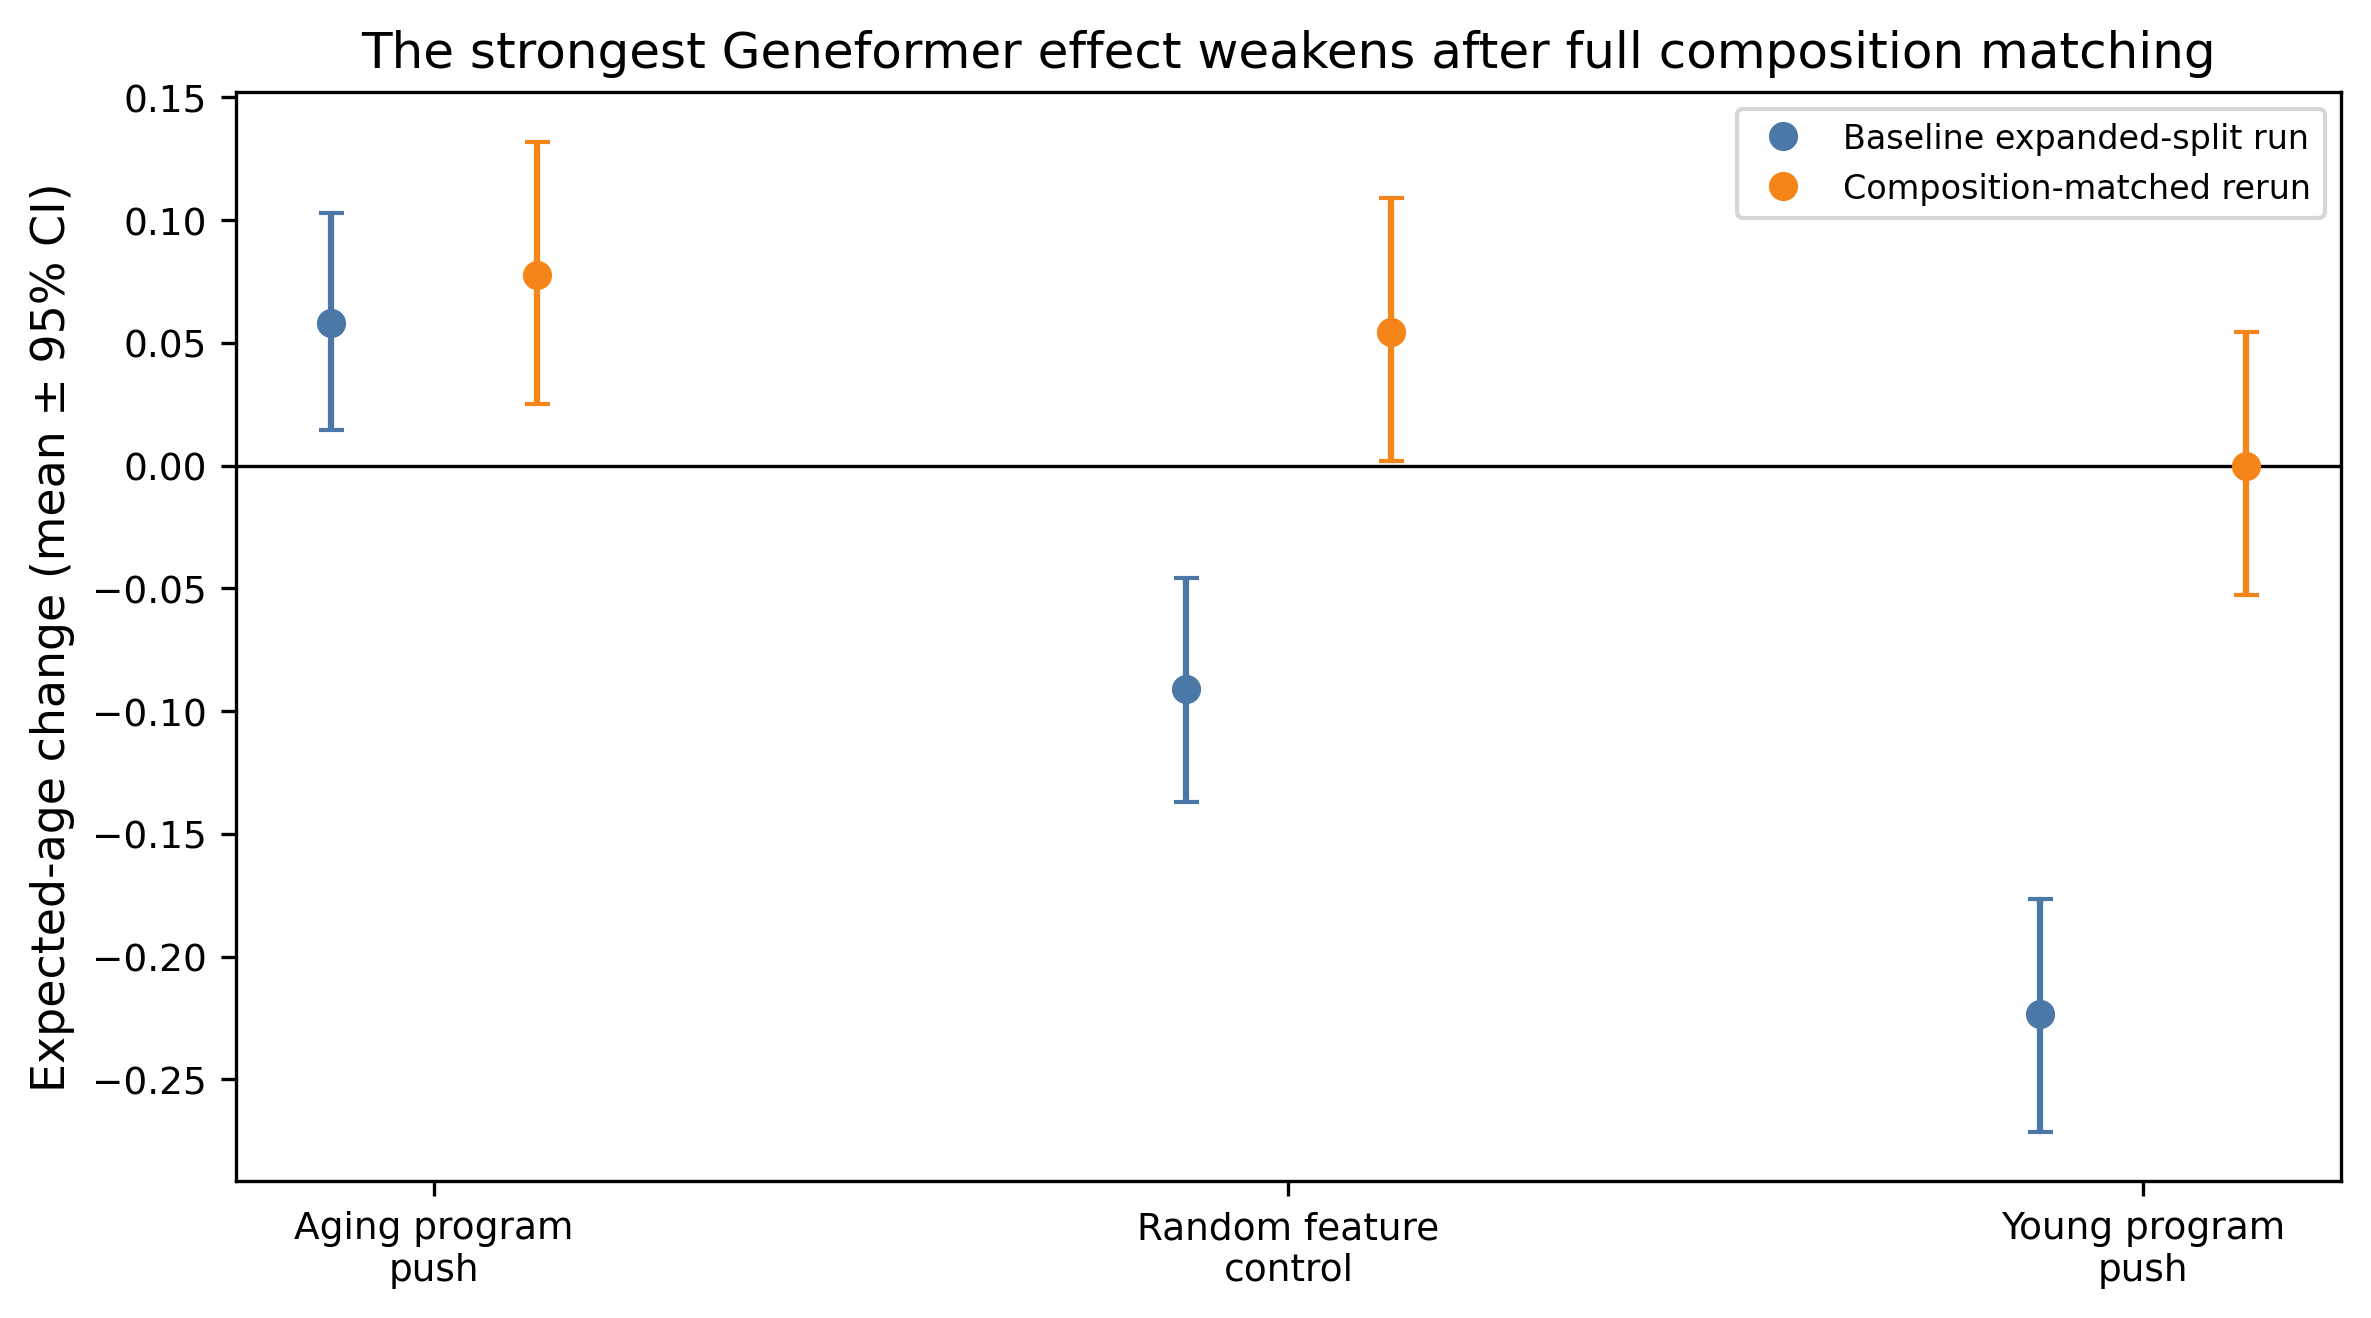
\includegraphics[width=0.78\textwidth]{figures/fig7_geneformer_bootstrap_stage9_vs_stage10.png}
\caption{Geneformer donor-bootstrap intervention effects before and after full composition matching. The aging-program push remains positive, but the overall directional structure becomes less clean once full matching is enforced.}
\label{fig:bootcompare}
\end{figure}

\subsection{Matched reruns do not reproduce the baseline claim}
A four-run composition-matched seed panel (seed42, 101, 202, 303) yielded:
\begin{itemize}
  \item \textbf{0/4} full strict replications,
  \item Geneformer directional-pattern criterion retained in \textbf{1/4} runs,
  \item unstable random/young intervention directional structure across seeds.
\end{itemize}

Table~\ref{tab:seedpanel} summarizes the panel-level strict outcomes.

\begin{table}[H]
\centering
\small
\caption{Composition-matched seed panel summary under the strict outcome criteria.}
\label{tab:seedpanel}
\begin{tabularx}{\textwidth}{Xcccc}
\toprule
\textbf{Run} & \textbf{$n_{\text{full strict}}$} & \textbf{Aging push} & \textbf{Random control} & \textbf{Young-program push} \\
\midrule
Baseline expanded-split run & 1 & positive & negative & negative \\
Composition-matched rerun, seed 42 & 0 & positive & positive & uncertain \\
Composition-matched rerun, seed 101 & 0 & uncertain & positive & positive \\
Composition-matched rerun, seed 202 & 0 & positive & positive & positive \\
Composition-matched rerun, seed 303 & 0 & positive & uncertain & uncertain \\
\bottomrule
\end{tabularx}
\end{table}

\section{Discussion}
A clear but mixed pattern emerged from the study. Frozen single-cell foundation models do contain aging-related structure, and some of that structure is biologically interpretable. We repeatedly recovered donor-aware sparse features, saw substantial cross-model overlap in inflammatory programs, and observed a strong cell-type-local monocyte signal in one of the two main immune-aging cohorts. This biological direction is plausible: inflammatory drift, NF-kappaB-linked signaling, senescence-associated secretory phenotypes, and immune remodeling are well-established features of aging biology \citep{franceschi2000inflammaging,furman2019chronic,ferrucci2018inflammageing,goronzy2019tcell,salminen2008nfkb,chien2011sasp,basisty2020secretome}. These findings are therefore more than generic age decoding. They indicate that frozen models can organize biologically meaningful aging-associated structure even without age-specific fine-tuning.

At the same time, the strongest global signal did not survive the most demanding control. The larger AIDA cohort yielded a Geneformer inflammation branch that remained convincing after split expansion, donor-threshold tightening, and donor-composition reweighting. However, once full composition matching was enforced and the analysis was repeated across multiple matched seeds, the full strict claim did not replicate. That result is not incidental. It is the central methodological message of the study.

\subsection{Interpretation for longevity-focused mechanistic research}
For longevity-focused mechanistic work, these results suggest a practical strategy:
\begin{itemize}
  \item Use frozen models first to test signal existence and feature interpretability.
  \item Promote candidate mechanisms only after donor-aware, cell-type-aware, and composition-aware replication.
  \item Distinguish \emph{model-specific interpretable signal} from \emph{cross-model robust mechanism}; these are not equivalent.
\end{itemize}

\subsection{Limitations}
Key limitations include limited donor support in some strata and external subsets, reduced power under strict within-cell-type constraints, sensitivity of final strict status to the specific composition-matched sample realization, and incomplete higher-budget composition-matched reruns due runtime constraints.

\section{Conclusion}
This study shows that frozen scGPT and Geneformer representations contain meaningful and interpretable aging-associated latent programs, with the clearest evidence concentrated in inflammatory biology. However, under repeated fully composition-matched forward-pass controls, the strongest global signal did not replicate at the strictest decision threshold. The most accurate summary is therefore: \textbf{promising mechanistic signal, but not yet a robust mechanism-level claim}.

The highest-value next step is a higher-power composition-matched consensus protocol, with larger matched cell budgets and pooled multi-resample decision rules, to determine whether the deep-dive inflammatory signal reflects a stable mechanism or a sampling-sensitive artifact.

\section*{Statements and Declarations}
\textbf{Funding:} The author received no specific funding for this work. \\
\textbf{Competing interests:} The author declares no competing interests. \\
\textbf{Author contributions:} The sole author conceived the study, designed the analyses, executed the computational work, interpreted the results, and wrote the manuscript. \\
\textbf{Ethics approval:} This study analyzed previously generated datasets and did not involve new recruitment or intervention on human participants within the present work. \\
\textbf{Consent to participate:} Not applicable. \\
\textbf{Consent for publication:} Not applicable. \\
\textbf{Data availability:} The public project repository includes the processed summary artifacts needed to reproduce the manuscript figures and tables. Access to the raw underlying single-cell datasets is governed by the original data providers; the repository documents dataset provenance and contains derived summary outputs only. \\
\textbf{Code availability:} The analysis code, manuscript source, figure-generation script, and reproducibility notes are available at \url{https://github.com/Biodyn-AI/longevity-mechinterp}. \\

\bibliographystyle{plainnat}
\bibliography{refs}

\end{document}
